\documentclass[11pt]{article}

\usepackage{common}
\usepackage{booktabs}
\usepackage{wrapfig}
\usepackage{titling}
\usepackage{titlesec}
\usepackage{float}
\usepackage[margin=0.99in]{geometry}

\titlespacing\section{0pt}{4pt}{2pt}
\setlength{\parskip}{0.35em}
\setlength{\droptitle}{-5em}
\pagestyle{plain}


\title{Practical 2: Classification\\ Classifying Malicious Software}
\author{\textit{Author names, emails, Camelot.ai usernames}\\
Fangli Geng, fgeng@g.harvard.edu, Camelot.ai fangligeng\\
Junran Yang, jyang3@gsd.harvard.edu, Camelot.ai junran}

\begin{document}


\maketitle{}


\noindent \textit{This is the template you should use for submitting your practical assignments. 
A full-credit assignment will go through each of these points and provide a thoughtful 
clear answer.  Note that the limit for the report is 4 pages, please prioritize quality over 
quantity in your submission.}

\section{Technical Approach}
\begin{enumerate}
\item \textbf{Feature Engineer}\\
The practical is to detect the malwares based on system calls recorded. The information we can get are system call tags and call attributes. We preserved the sequence of system calls by generating the 4-grams for the call tags, since the sequence may infer the patterns of certain program behavior and anomaly behaviors usually indicate malwares. We also extract certain type of system call attributes, such as filename, url, keys, etc. We found some attributes are very suspicious, for example, "maxtrox.txt" always indicates the VB Malware and "GrayPigeon\_Hacker.com.cn" always indicates the Hupigon Malware. In addition, we also take total processes and threads number into account.

To analyze the system call tags (including 4-grams, 29,813 features in total) and suspicious attributes (110,465 features in total), we tried 2 ways: using either the count or the TF-IDF (term frequency – inverse document frequency) [System Call-based Detection of Malicious Processes.pdf]. The TF-IDF value increase proportionally to the number of times a word appears in the file and is offset by the frequency of the word among all files, which helps to adjust for the fact that some words appear more frequently in general.

To utilize TF-IDF, we first generated a giant string, which contains system call tags, 4-grams, and suspicious system call attributes, for each file in both train and test set. We then extracted the TF-IDF values from the train set by using sklearn.feature\_extraction.text.TfidfVectorizer, and at last applied it to the test set. 

\item \textbf{Feature Selection}\\
Since we have roughly 140,000 features but with only a little more than 3,000 data points, it's easy to cause our model to over-fit the data. To avoid over-fitting, we use sklearn SelectFromModel and sklearn.ensemble.RandomForestClassifier to reduce features and use cross-validation to determine the features we want to keep. To be specific, we ran a loop to continuous drop features, which importance is less than 0.1 times mean of all features' importance, until all features has similar importance. At the same time we compared the score from 5 fold cross-validation in each iteration. The highest score happened with around 5000 features, which is 1/20 of original feature size. 
\item\textbf{Model Selection}\\
Regarding the classification tasks and limited number of data points, we first selected several models to start with, including RandomForestClassifier, sklearn.svm.SVC, sklearn.svm.LinearSVC and sklearn.linear\_model.SGDClassifier with default hyper-parameters. The RandomForestClassifier behaved superior that other models:
RandomForestClassifier: 0.78105
SVC: 0.57211
LinearSVC: 0.76789
SGDClassifier: 0.77158

In addition, we found the data distribution is heavily imbalanced which affects the models' performance. I (fangli. Antonio had a similar approach, a.k.a. sequential predictions) tried a 2-steps approach, which gave approximate 0.02 boost over similar Random Forest Classifier settings (0.81211 vs 0.79263). We grouped the classes into 4 "categories": None, Swizzor, VB, Others. We did classification over the "categories" first and then over the rest minor malwares. We also applied Neural Network to 2-steps approach but it can't beat Random Forest Classifier (0.79105 vs 0.81211)

We found that we had only collected information from every other thread caused by a bug in started example. Later experiment is based on the fixed feature collection, but given the limit of time, we only used tags and 4-grams count. With similar Random Forest Classifier settings (1-step), less features (no suspicious system call attributes) but preciser information, we got 0.15 boost (0.80789 vs 0.79263).

Instead of repeating the 2-steps with new set of features, we started a new model experimenting, inspired by a Microsoft Malware Classification Challenge (BIG2015)\footnote{https://www.kaggle.com/c/malware-classification/discussion/13897}, which utilized xgboost and semi-supervised method to detect malwares from assembly code. As Gradient Boosting focuses more on reducing the bias than variance, which is different from what Random Forest classifier does. After grid searching for hyperparameters, the highest accuracy we got by xgboost is 0.82526. Furthermore, We tried semi-supervised Gradient Boosting, aiming to further reduce the bias of the model and incorporate information from test dataset into training dataset. We first generate pseudo labels of test set by choosing the max probability of our best model. Then we predict the test set again in a cross validation fashion with both train data and test data.
For example, the test data set is split to 4 part A, B, C and D. We use the entire training data, and test data A, B, C with their pseudo labels, together as the new training set and we predict test set D. The same method is used to predict A, B and C. However, this approach didn't provide us decent results. We suspect the relatively low accuracy in the prediction set (0.82526) provided more inaccurate information than that it could offer to reduce bias. 
\end{enumerate}

\textit{How did you tackle the problem? Credit will be given for:}

  \begin{itemize}
  \item \textit{Diving deeply into a method (rather than just trying
    off-the-shelf tools with default settings). This can mean 
    providing mathematical descriptions or pseudo-code.}
  \item \textit{Making tuning and configuration decisions using thoughtful experimentation.  
    This can mean carefully describing features added or hyperparameters tuned.}
  \item \textit{Exploring several methods. This can contrasting two approaches
    or perhaps going beyond those we discussed in class.}
  \end{itemize}

  \noindent \textit{Thoughtfully iterating on approaches is key.
  If you used existing packages or referred to papers or blogs for ideas,
  you should cite these in your report. }

  \begin{table}
    \centering
    \begin{tabular}{@{}lll@{}}
%      \toprule
      &\multicolumn{2}{c}{Mention Features  } \\
      & Feature & Value Set\\
      \midrule
      & Mention Head & $\mcV$ \\
      & Mention First Word & $\mcV$ \\
      & Mention Last Word & $\mcV$ \\
      & Word Preceding Mention & $\mcV$ \\
      & Word Following Mention & $\mcV$\\
      & \# Words in Mention & $\{1, 2, \ldots \}$ \\
      & Mention Type & $\mathcal{T}$ \\
      \bottomrule
      
    \end{tabular}
    \caption{Feature lists are a good way of illustrating problem specific tuning.}
  \end{table}



\section{Results}
\textit{This section should report on the following questions: }

\begin{itemize}
\item \textit{Did you create and submit a set of
  predictions? }

\item  \textit{Did your methods give reasonable performance?  }
\end{itemize}

\noindent \textit{You must have \textit{at least one plot or table}
that details the performances of different methods tried. 
Credit will be given for quantitatively reporting (with clearly
labeled and captioned figures and/or tables) on the performance of the
methods you tried compared to your baselines.}

\begin{table}
\centering
\begin{tabular}{cccccccc}
 \toprule
 Rank & max\_depth & eta & min\_child\_weight & colsample & cv mean error & best num\_round & final score\\
 \midrule
  1 & 4 & 0.15 & 1 & 0.5 & 0.0933316 & 49 & 0.82158\\
  2 & 6 & 0.2 & 1 & 1 & 0.093334 & 25 & 0.811054\\
  3 & 4 & 0.1 & 1 & 0.5 & 0.093983 & 68 & 0.82526\\
  4 & 4 & 0.15 & 2 & 0.5 & 0.094306 & 54 & - - -\\
  5 & 6 & 0.15 & 1 & 1 & 0.0949526 & 31 & - - -\\
 \bottomrule
\end{tabular}
\caption{\label{tab:results} Result tables for the best 5 cross-validation scores by Gradient Boosting with grid search}
\end{table}

Table 2 shows the best 5 cross-validation scores by Gradient Boosting with grid search. The hyper-parameters we tuned were max\_depth (the maximum depth of a tree, same as GBM, set as 2, 4, 6), eta (analogous to learning rate in GBM, set as 0.05, 0.1, 0.15, 0.2),  min\_child\_weight (defines the minimum sum of weights of all observations required in a child, set as 1, 2), colsample\_bytree (denotes the subsample ratio of columns for each split, in each level, set as 0.5, 1). Those 48 configurations were selection based on what we found people commonly used. We also tested models with higher and lower rounds numbers, which were different from what were the best indicated by cross-validation. Then we found it would give us worse performance by using those round numbers, compared to that from best round numbers setting given by cross validation.


\begin{figure}[H]
\minipage{0.5\textwidth}
  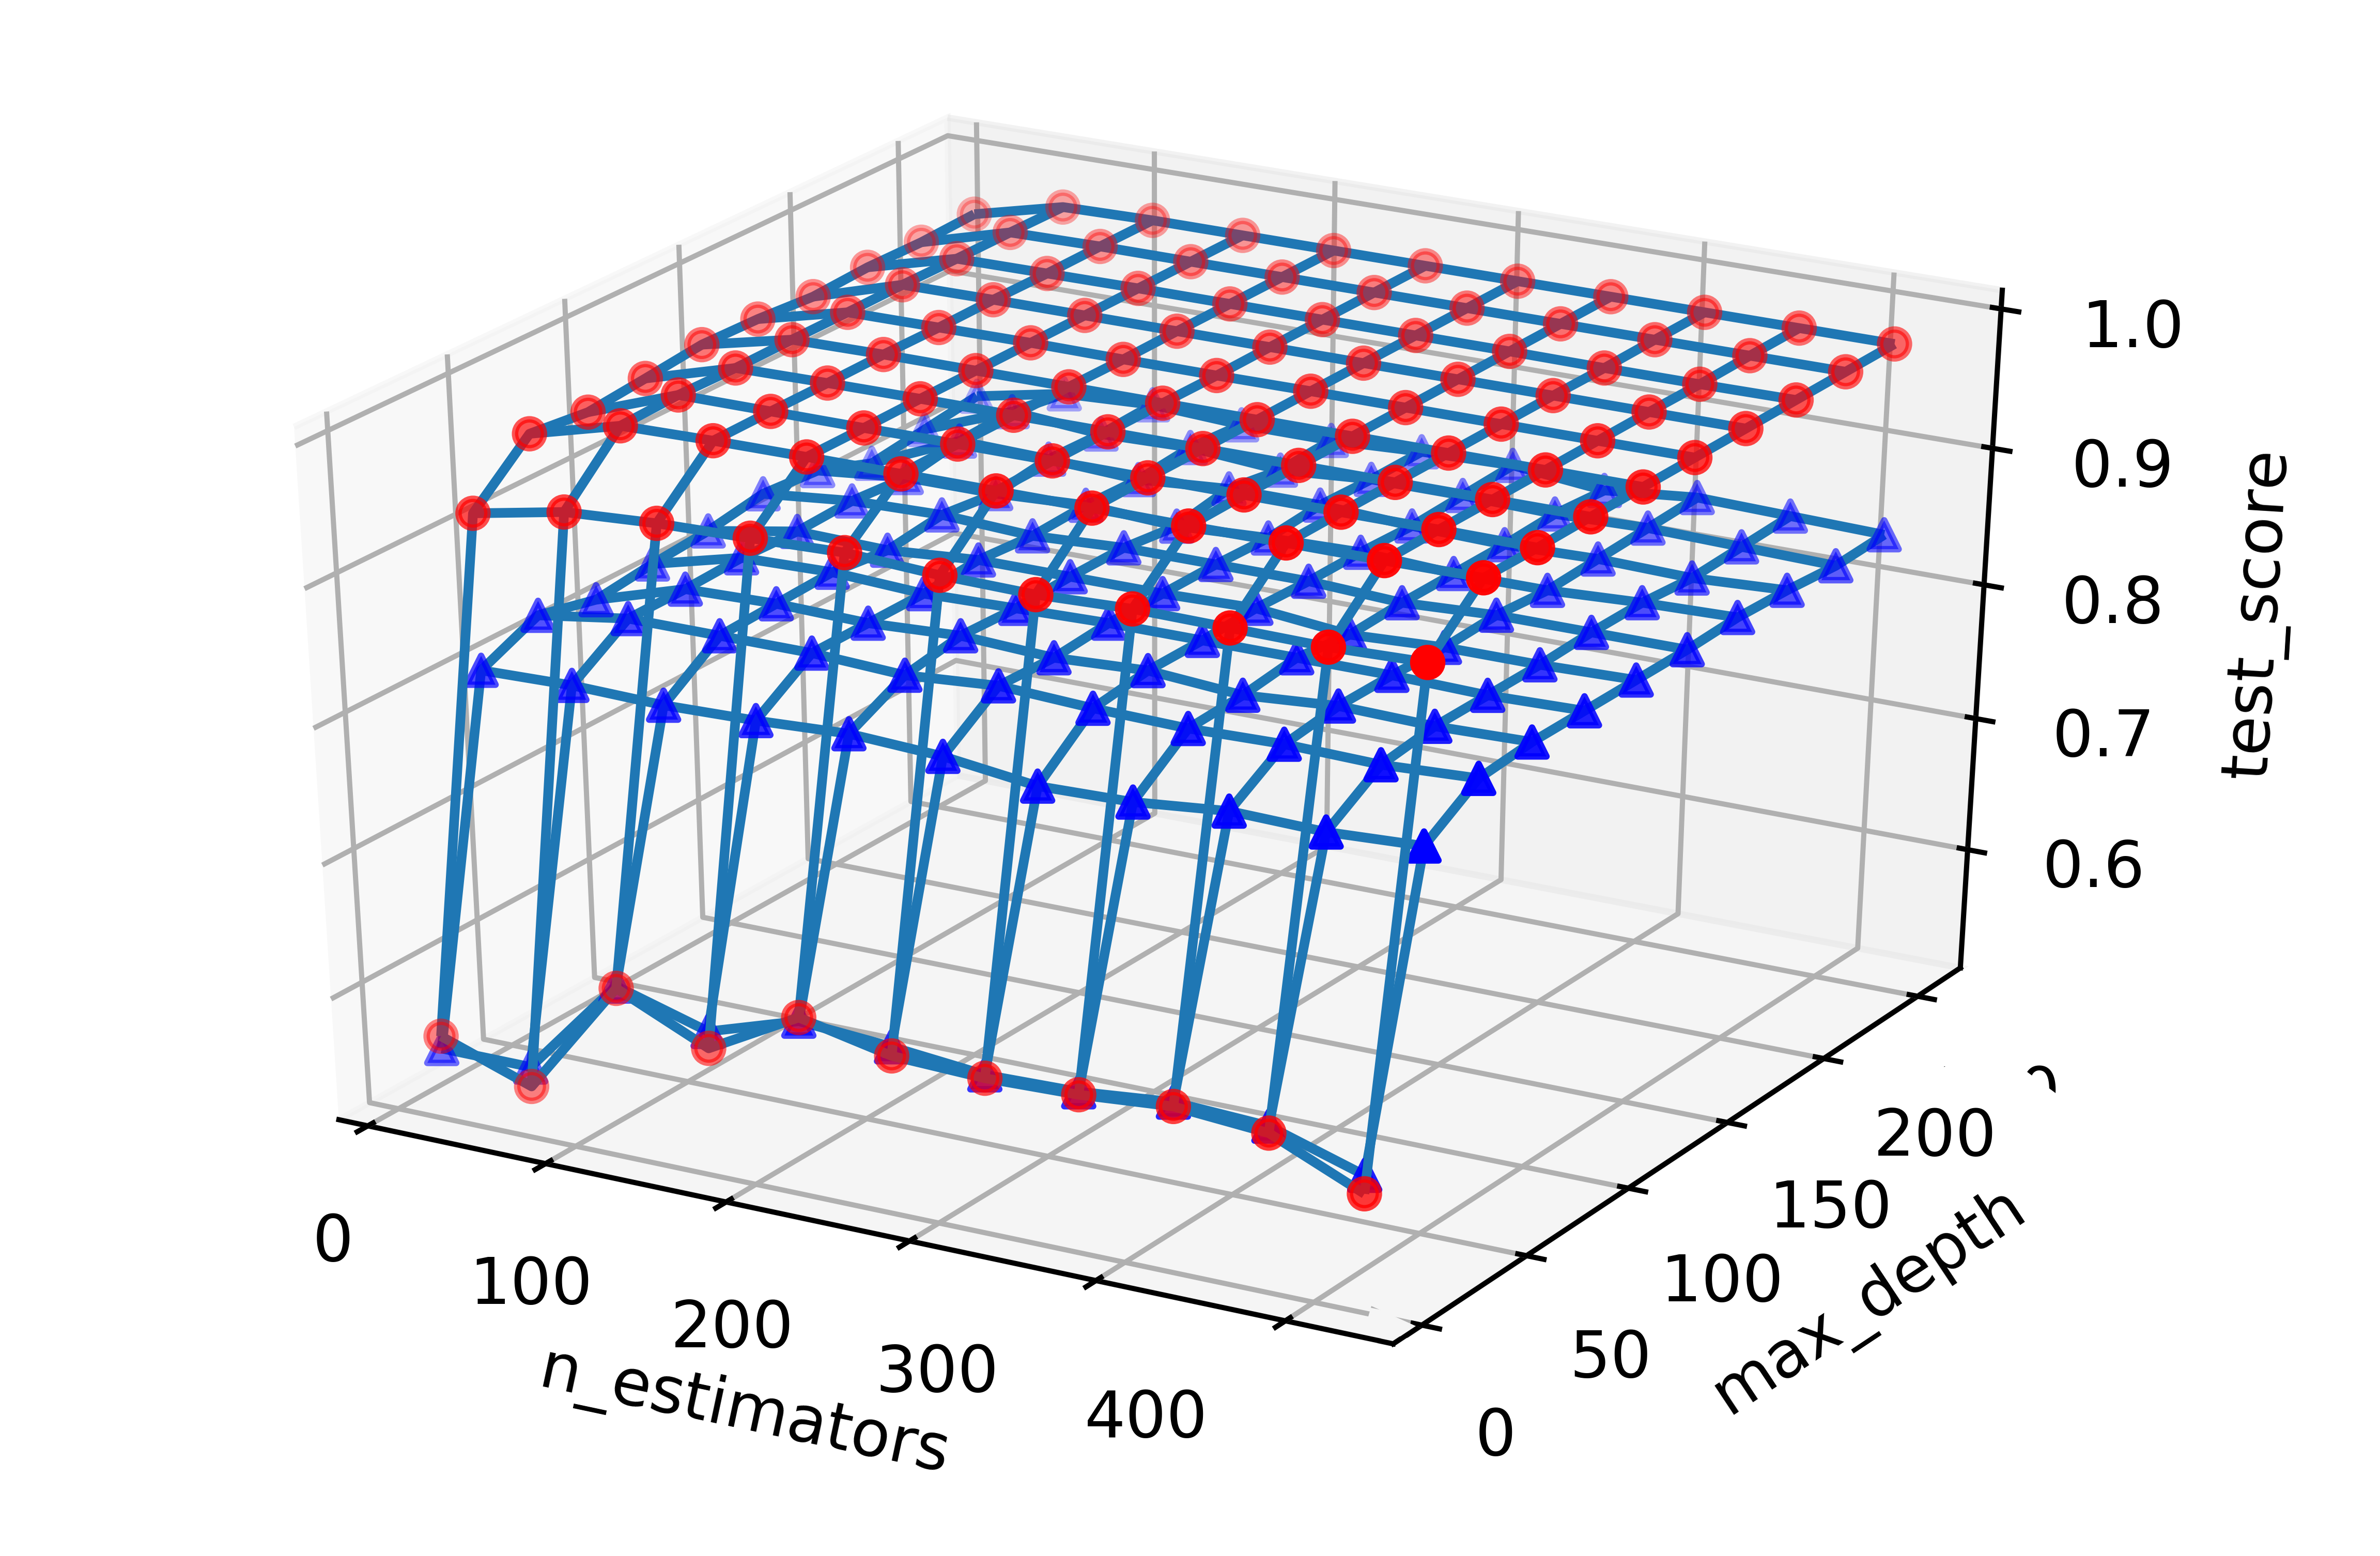
\includegraphics[width=\linewidth]{hyperparameter_tuning_1}
  \caption{Max depth range from 10 to 235, and number of estimators range from 10 to 460.}
  \label{fig:results}
\endminipage\hfill
\minipage{0.5\textwidth}
  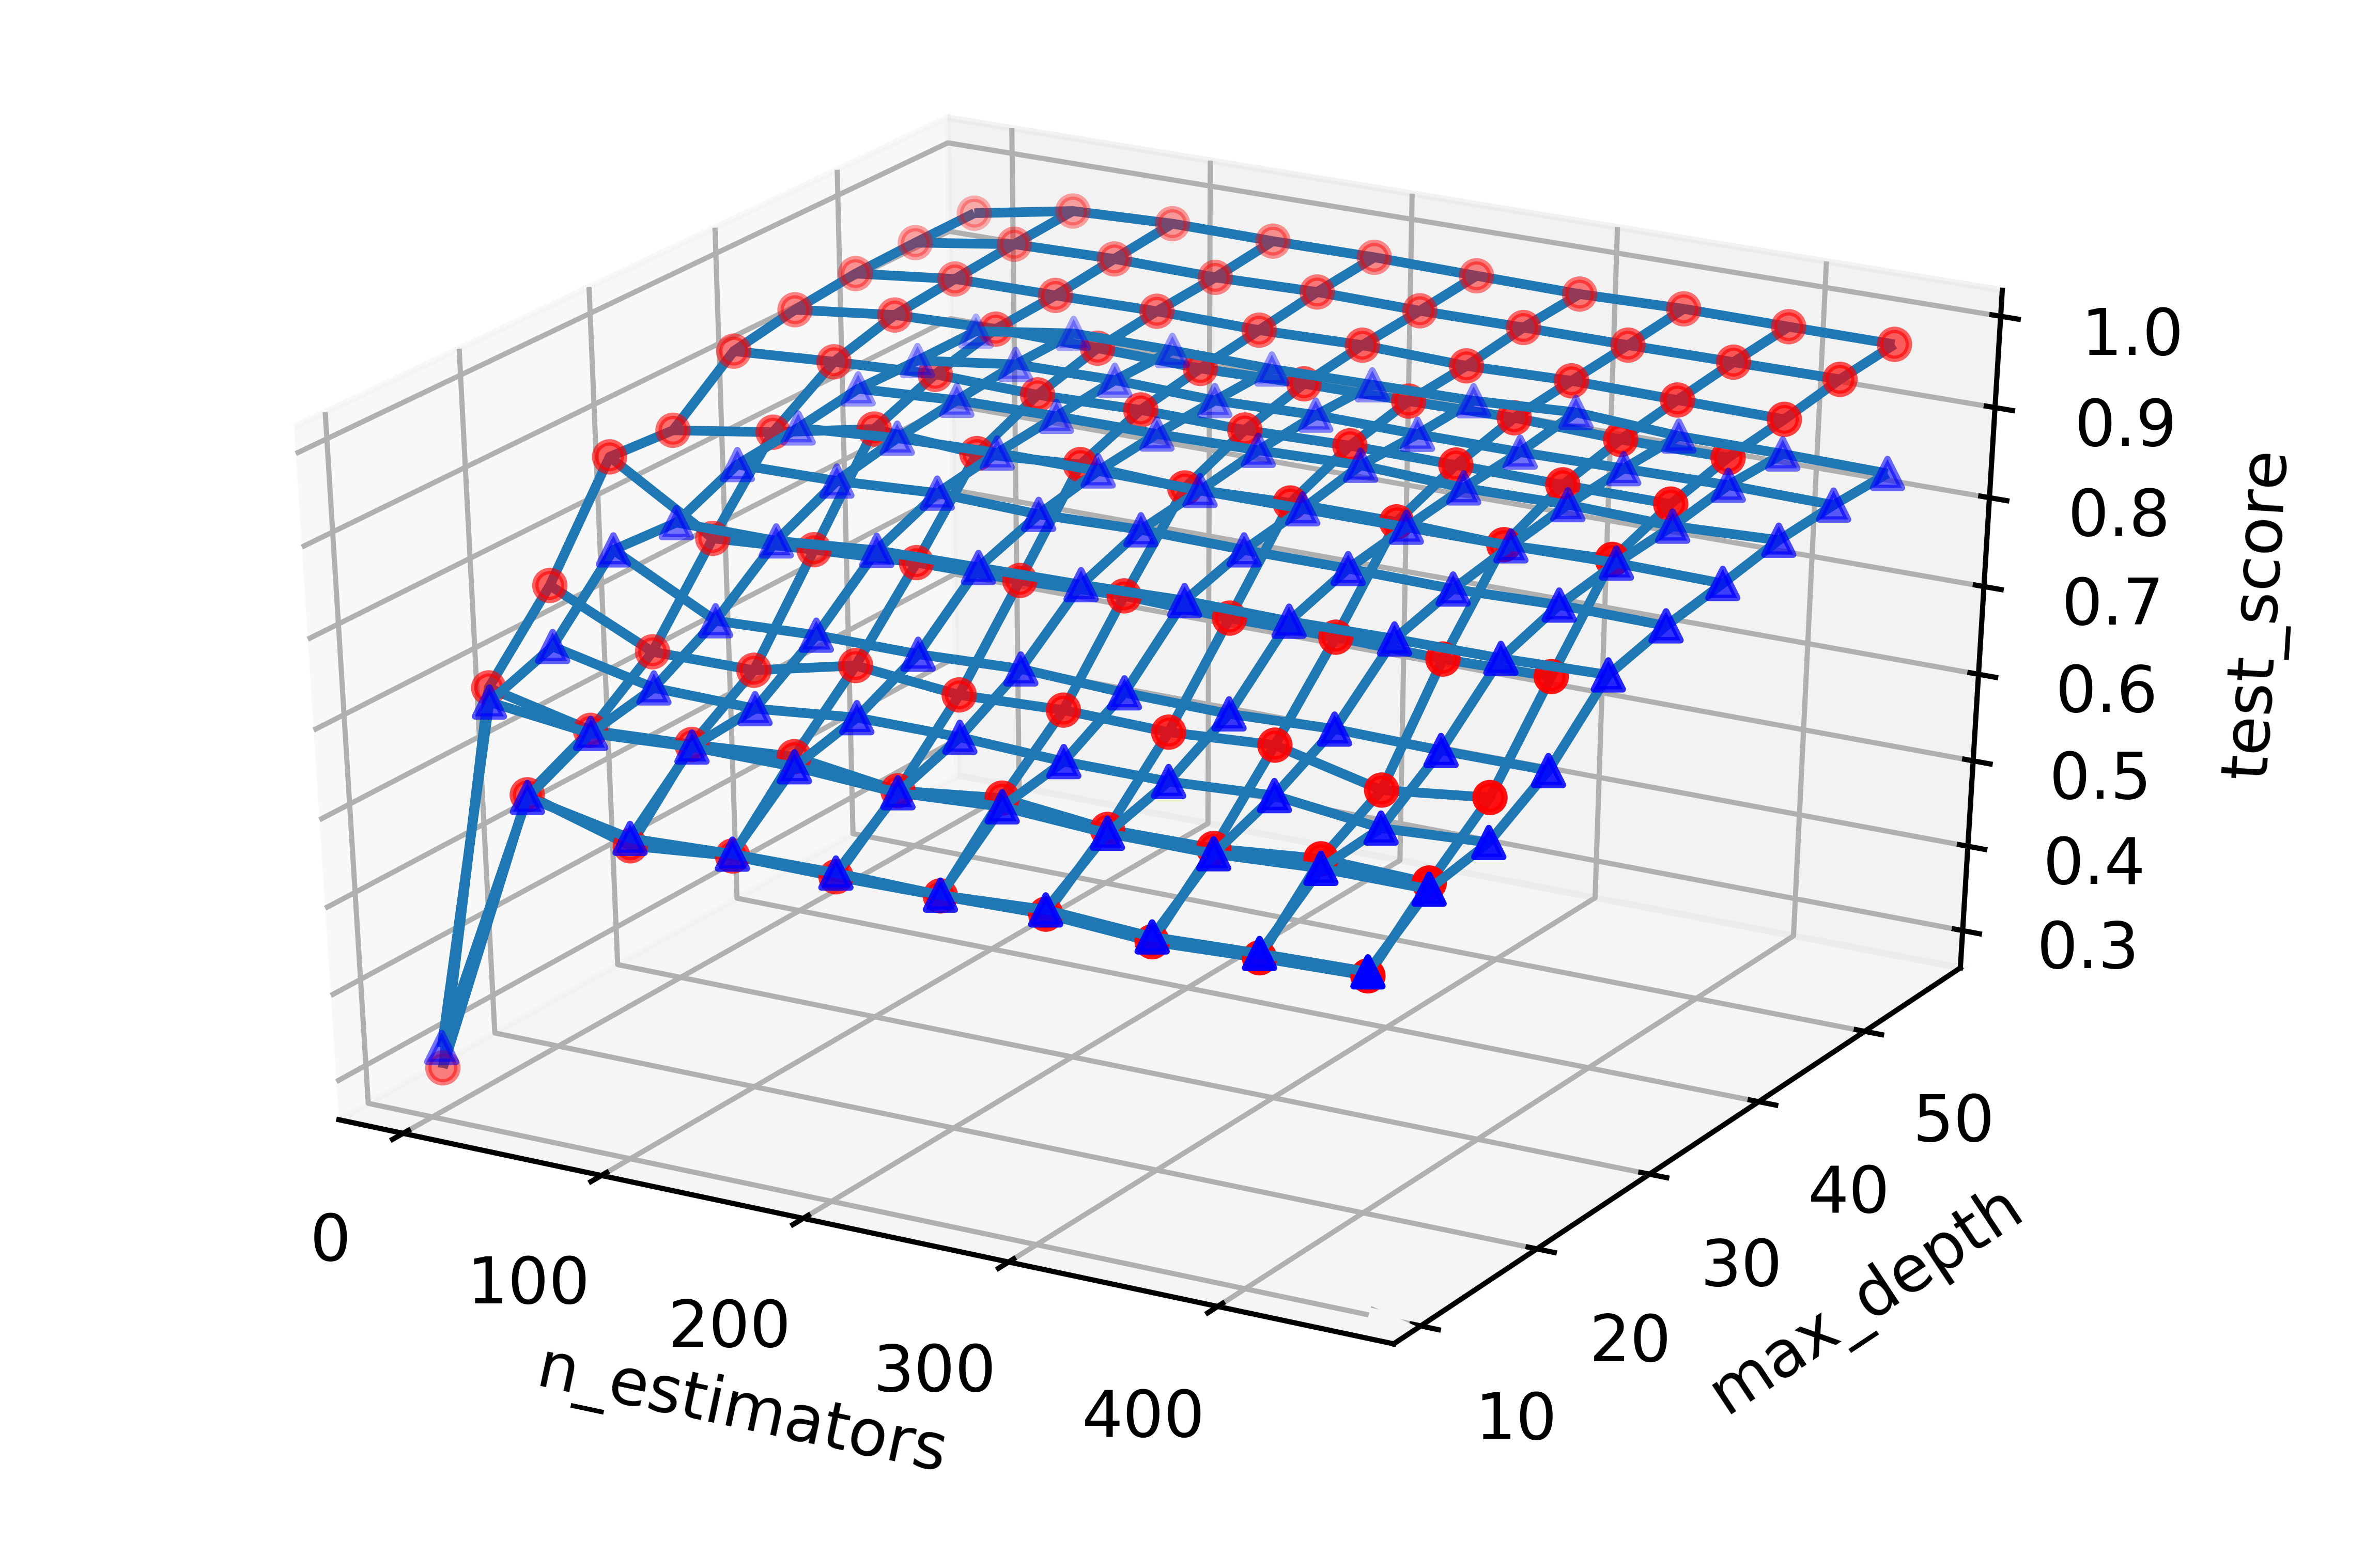
\includegraphics[width=\linewidth]{hyperparameter_tuning_2}
  \caption{Max depth range from 10 to 45, and number of estimators range from 10 to 460.}
  \label{fig:results}
\endminipage\hfill
\minipage{1\textwidth}
  \begin{center}
  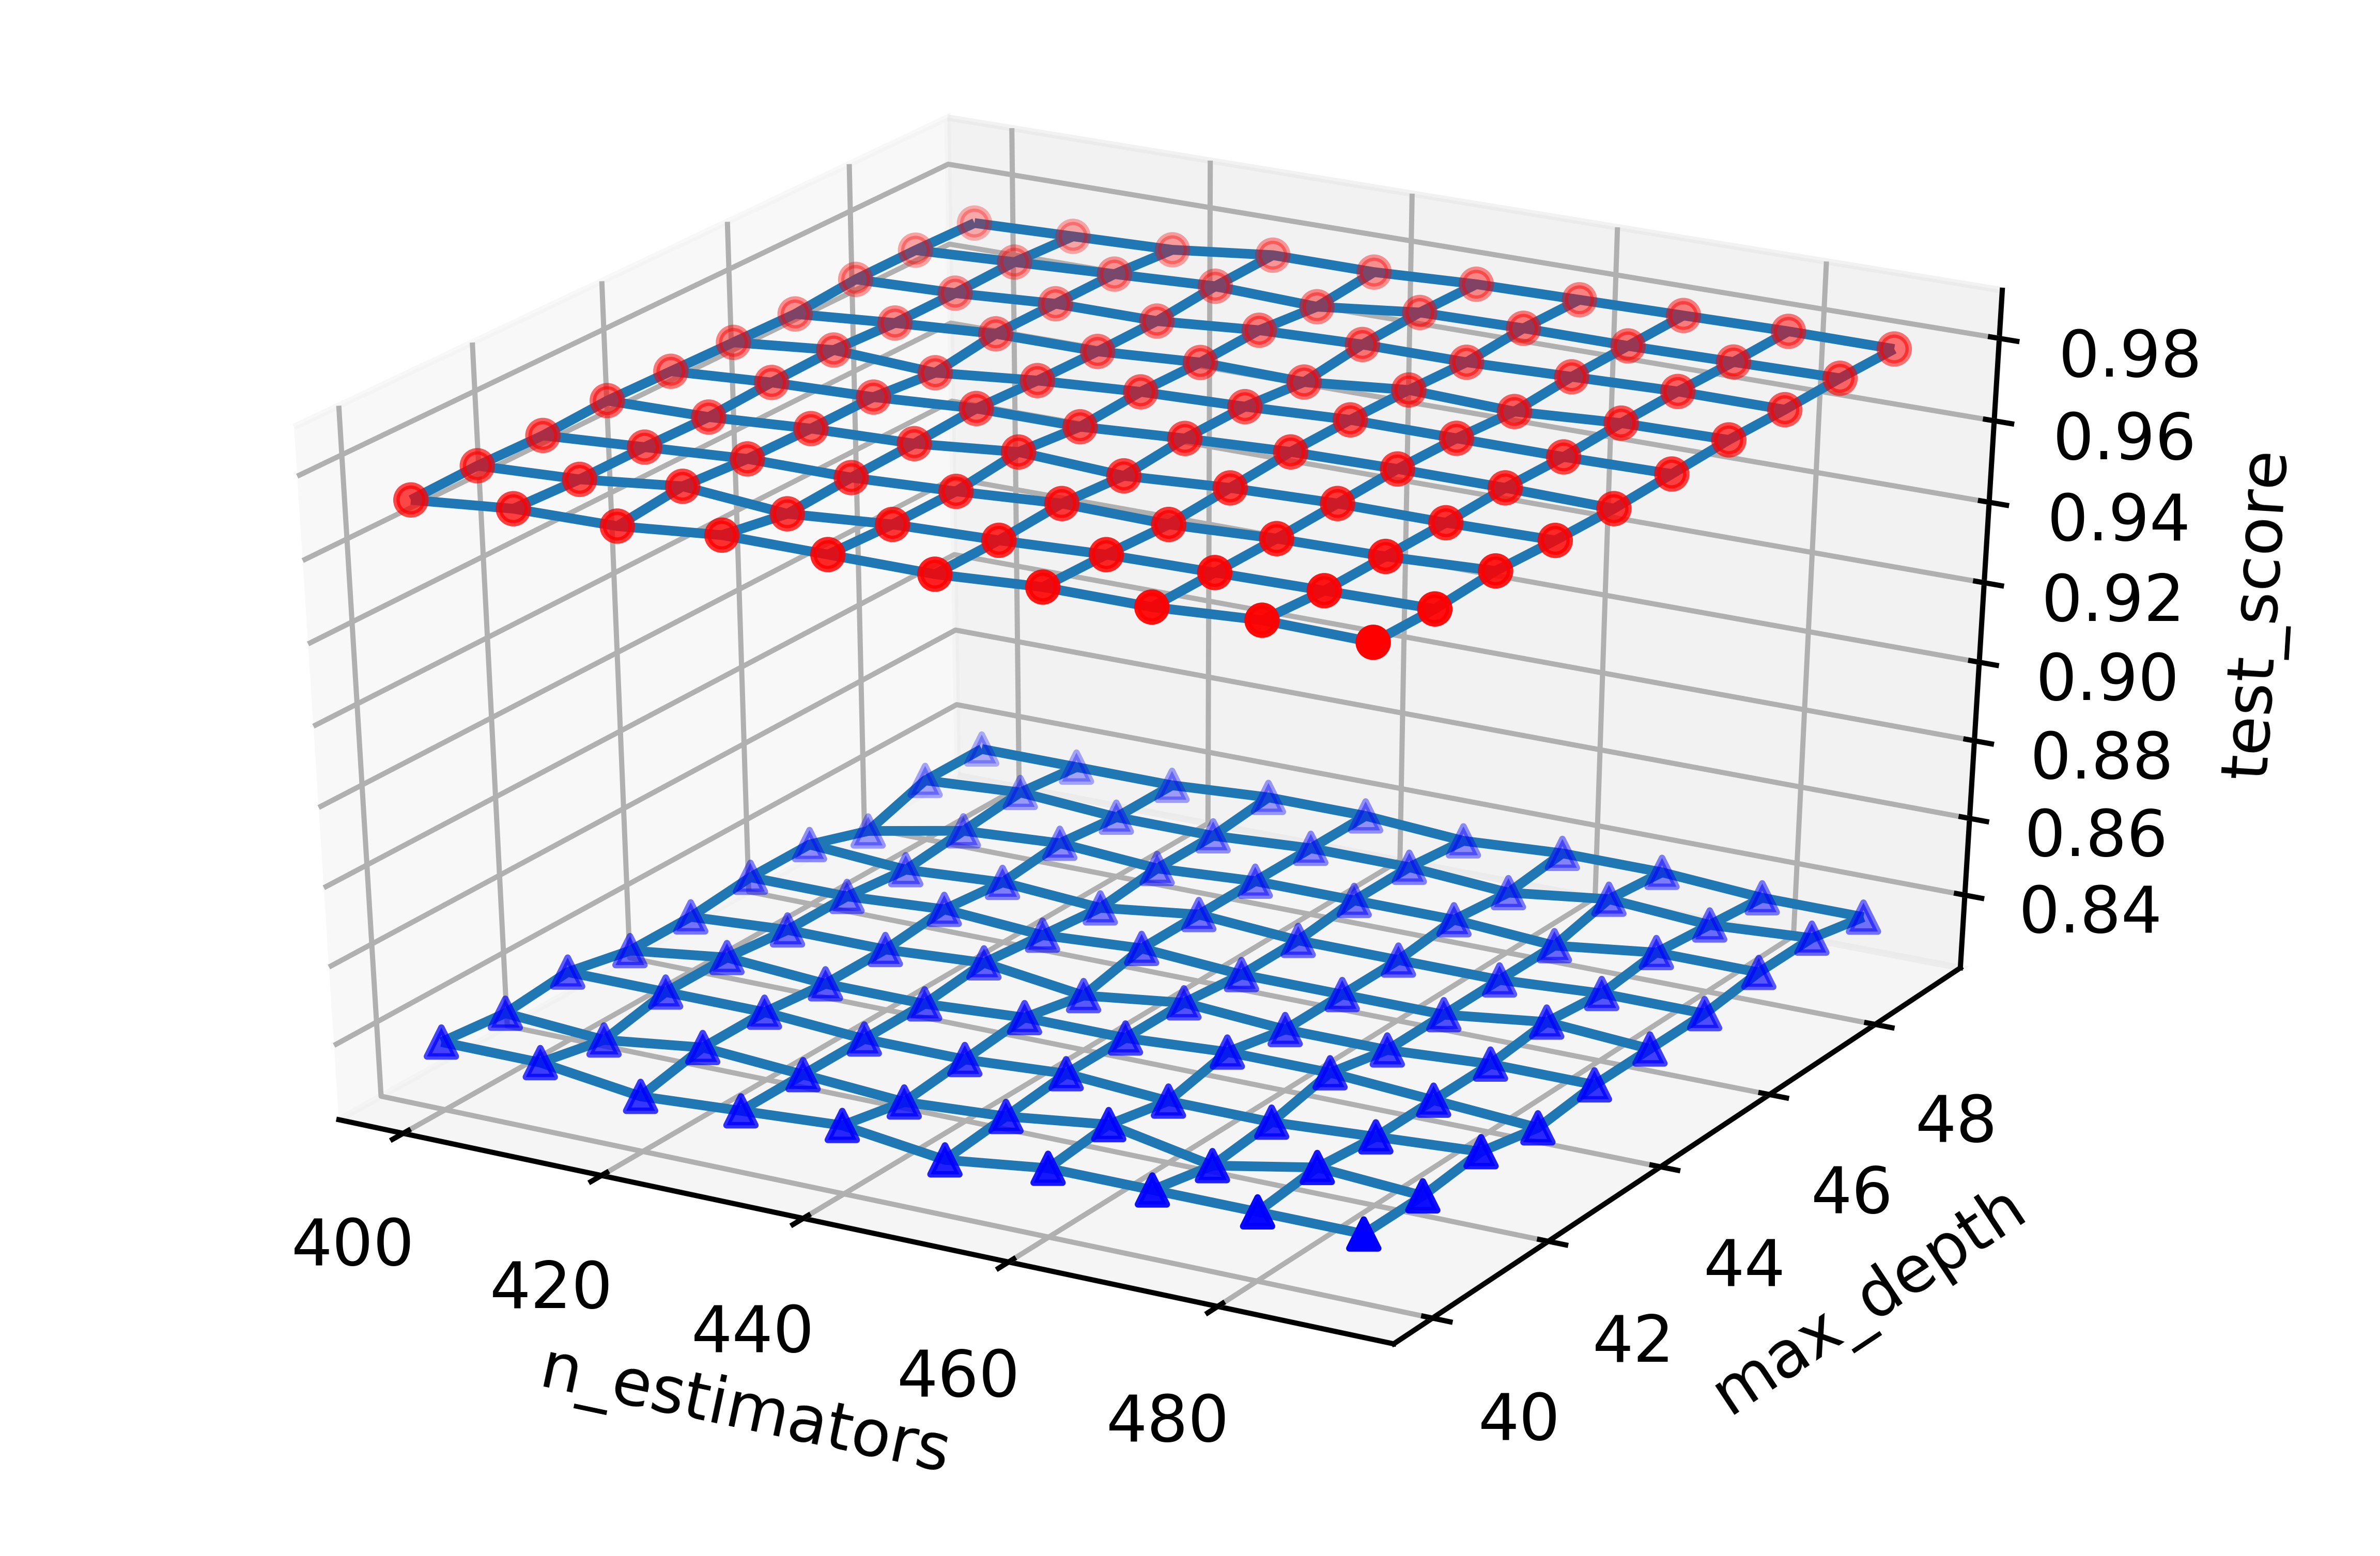
\includegraphics[width=0.5\linewidth]{hyperparameter_tuning_3}
  \caption{Max depth range from 40 to 49, and number of estimators range from 400 to 490.}
  \label{fig:results}
  \end{center}
\endminipage
\end{figure}

Figure 1-3 show the hyper parameter tuning process for random forest model. We first ran the experiment in a rough region: max\_depth range from 10 to 235 with a step of 25, while n\_estimators range from 10 to 460 with a step of 50. From this experiment we found out that when depth is larger than 60, the increasing depth of the decision tree no longer contributes to train score or test score. That is because we only have a training set of around 3000 samples, and making the tree deeper than the square root of number of samples could not contribute to the accuracy of the decision trees. \\
Then we ran 2 experiments with finer sampling. We found out from the results that we should make the depth as close to the square root of number of samples as possible, while choosing number of estimators to be around 400, since larger number of estimators no longer improve the performance of the model significantly. 

\section{Discussion} 


\textit{End your report by discussing the thought process behind your
analysis. This section does not need to be as technical as the others 
but should summarize why you took the approach that your did. Credit will be given for:
}
  \begin{itemize}
  \item \textit{Explaining the your reasoning for why you seqentially chose to
    try the approaches you did (i.e. what was it about your initial
    approach that made you try the next change?).  }
  \item Explaining the results.  \textit{Did the adaptations you tried improve
    the results?  Why or why not?  Did you do additional tests to
    determine if your reasoning was correct?  }
  \end{itemize}
 
First, we focused on new feature generating process. We came up with 1-gram, 2-gram, 3-gram, 4-gram, 10-gram of system call tags, useful system call attributes we identified, TFIDF for feature scaling. Then, based on the classification task we were give and the limited sample size we faced, we decided to test several different basic models (Random Forest Classifier, C-Support Vector Classifier, Linear-Support Vector Classifier, Stochastic Gradient Decent classifier) with different subsets of those data. With the results from those experiments, we decided to narrow down to Random Forest and deeply tune the hyperparameters to achieve best possible results. We further improved the Random Forest approach by 2-step classification, in order to capture more detail information in the Malware categories with low percentage. As the results is still not ideal with a 0.816 accuracy score, we did The accuracy can be higher with full feature scaled by TF-IDF. Furthermore, aiming to reduce the bias of the overfitting models, we took Gradient Boosting approach, which ended up giving the best accuracy among all the models we tested. 

If there were more time to pursue better estimates, we would try to resample from the original data set as new training sets to reduce bias, and further tune semi-supervised Gradient boosting models. We also consider to create a 2-step Gradient Boosting approach to capture more detail information in the small malware categories as what we did for Random Forest.

\end{document}

